
\section{Intermediate vector bosons}
$\mathcal{L}_{4F}$ provides an excellent description of low-energy charged current weak interactions. But it runs into problems at higher energies.
\subsection{Unitarity}
\subsubsection{Example:  $\nu_\mu e^- \to \mu^- \nu_e$}
We can write the matrix element for this process
\newline
\begin{equation}
\begin{split}
\mathcal{M} &= -i \frac{G_F}{2} \bar{v}(q^\prime)\gamma_\mu(1-\gamma^5)u(p) \bar{u}(p^\prime)\gamma^\mu(1-\gamma^5)u(q) \\
 \frac{1}{2}\sum_{spins}|\mathcal{M}|^2 &= \frac{1}{4} G_F\ tr\bigg(\slashed{q}^\prime \gamma_\mu(1-\gamma^5)(\slashed{p}+m_e)\gamma_\nu(1-\gamma^5)\bigg) \\
 &\times tr\bigg((\slashed{p}^\prime + m_\mu)\gamma^\mu(1-\gamma^5)\slashed{q}\gamma^\nu(1-\gamma^5)\bigg)\\
 &= 64\ G_F^2(p \cdot q)(p^\prime \cdot q^\prime) \\
 &= 16\ G_F^2(s-m_e^2)(s-m_\mu^2)
\end{split}
\end{equation}
where we used $s = (p+q)^2 = (p^\prime + q^\prime)^2 = m_e^2 + 2 p \cdot q = m_\mu^2 + 2p^\prime \cdot q^\prime$. 
\begin{wrapfigure}{l}{0.4\linewidth}
  \centering
  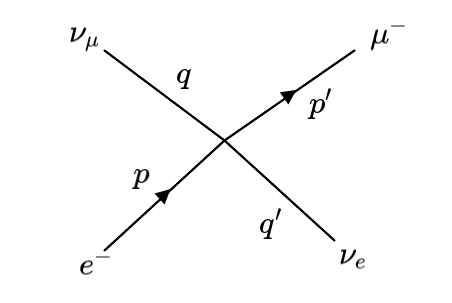
\includegraphics[width=\linewidth]{figs/diag_5.png}
\end{wrapfigure}
In the centre of mass frame, ignoring masses (i.e. at high energy)
\begin{equation}
\bigg(\frac{d\sigma}{d\Omega}\bigg)_{CoM} = \frac{1}{64\pi^2s}\frac{1}{2}\sum_{spins}|\mathcal{M}|^2 = \frac{1}{4\pi}G_F^2s.
\end{equation}
Using $s=4E^2$, $d\Omega = 2\pi\ d(\cos\theta)$,
\begin{equation}
\frac{d\sigma}{d\cos\theta} = \frac{2G_F^2}{\pi}E^2.
\end{equation}
Compare this with, for example, the equivalent result for $e^+e^- \to \mu^+\mu^-$:
\begin{equation}
\frac{d\sigma}{d\cos\theta} = \frac{\alpha^2}{4\pi E^2}(\cos^4\theta/2 + \sin^4\theta/2)
\end{equation}
QED cross-sections scale as $1/E^2$ as $E \to \infty$. But Fermi theory cross-sections rise as $E^2$ as $E \to \infty$. This is a disaster! $|\mathcal{M}|^2$ is a probability, so it must be bounded. It can be shown quite generally that any cross section can be decomposed using the partial wave approximation:
\begin{equation}
\sigma = \frac{4\pi}{E^2}\sum_j(2j+1)|f_j|^2
\end{equation}
where $|f_j|^2 \leq 1$, which follows from $S^\dagger S =1$. In other words, we define contributions $\sigma_j \leq \frac{4\pi}{E^2}(2j+1)$. We can see from dimensional arguments that the Lagrangian leads to unitarity violation. $[G_F]=-2$ and $[\sigma]=-2$ so because $E$ is the only scale then $\sigma \sim G_F^2E^2$. We can see that as $E \to \infty$ we will end up with infinite cross sections, violating unitarity. 
%
\subsection{Renormalisability}
%
We need to draw all the possible Feynman diagrams. Consider, for example, $\nu_e\bar{\nu}_\mu \to \nu_e\bar{\nu}_\mu$.
\begin{wrapfigure}{l}{0.4\linewidth}
  \centering
  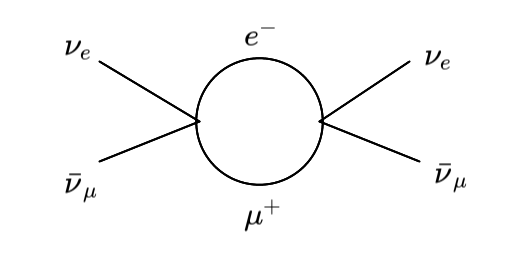
\includegraphics[width=\linewidth]{figs/diag_6.png}
\end{wrapfigure}
The vertex receives contributions from loop diagrams like the one shown here. But the loop gives contributions to the amplitude of the form
\begin{equation}
\sim \int d^4k \frac{\slashed{k}}{k^2}\frac{\slashed{k}}{k^2} \sim \int \frac{d^4k}{k^2}.
\end{equation}
In other words, the loop leads to quadratic divergences. But there is no $\bar{\nu}\nu\bar{\nu}\nu$ term in $\mathcal{L}$ to cancel this.
%
\subsection{Power counting}
%
Let's take QED as an example. Consider a graph with $L$ loops, $I_F$ fermion lines and $I_B$ photon lines. Considering the structure of contributions from Feynman rules, we can define the "superficial degree of divergence", $D$, to be
\begin{equation}
D = 4L - I_F - 2I_B.
\end{equation}
The logic here is that each loop contributes a $\int d^4k$ term, i.e. +4 powers of $k$. This gives the $4L$ term. Likewise, each fermion propagator contributes $\frac{\slashed{k}}{k^2}$, i.e. -1 powers of $k$, and each boson propagator contributes $\frac{1}{k^2}$, i.e. -2 powers of $k$. If $D \geq 0 $ then we would naively expect the graphs to lead to divergences. We can also impose the general result from graph theory that for $L$ loops, $I$ internal lines and $V$ vertices:
\begin{equation}
L = I - V + 1.
\end{equation}
The proof is by induction and left as an exercise. This means that
\begin{equation}
D = 2I_B + 3I_F - 4V + 4.
\end{equation}
Moreover, for QED we have the additional ammunition that there is only one type of vertex, joining two fermions and a photon. So, counting the ends of lines and labelling external lines $E$:
\begin{equation}
\begin{split}
&2I_B + E_B = V \\
&2I_F + E_F = 2V \\
\text{so } D &= V-E_B + \frac{3}{2}(2V-E_F) - 4V + 4 \\
&= 4 - E_B - \frac{3}{2}E_F
\end{split}
\end{equation}
i.e. $V$ cancels! $D$ is independent of $V$ and the only divergent graphs ($D \geq 0$) have corresponding counterterms which can regulate the divergences. The table enumerates the cases for QED where $D \geq 0$, explaining how each of these terms does in fact not lead to a divergence in this instance.
\begin{table}[h!]
\begin{tabular}{llll}
$E_B$ & $E_F$ & Diagram                                                 & Comments                                                                                              \\
\hline
2     & 0     & 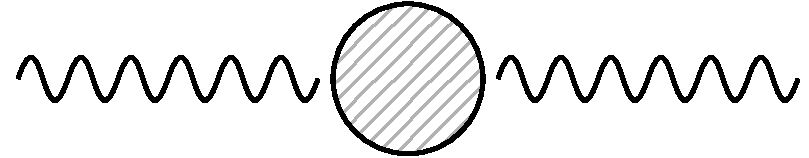
\includegraphics[scale=0.2]{figs/pc1.pdf} & $F_{\mu\nu}F^{\mu\nu}$, i.e. $Z_3$                                                                         \\
3     & 0     & 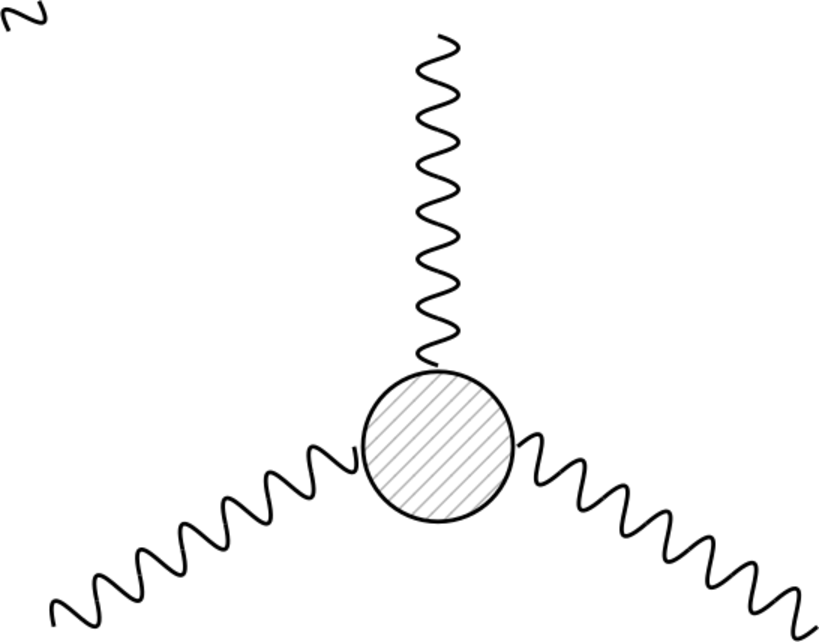
\includegraphics[scale=0.2]{figs/pc2.pdf}  & Photon is odd under $C$ so this gives 0 contribution                                                    \\ 
4     & 0     &  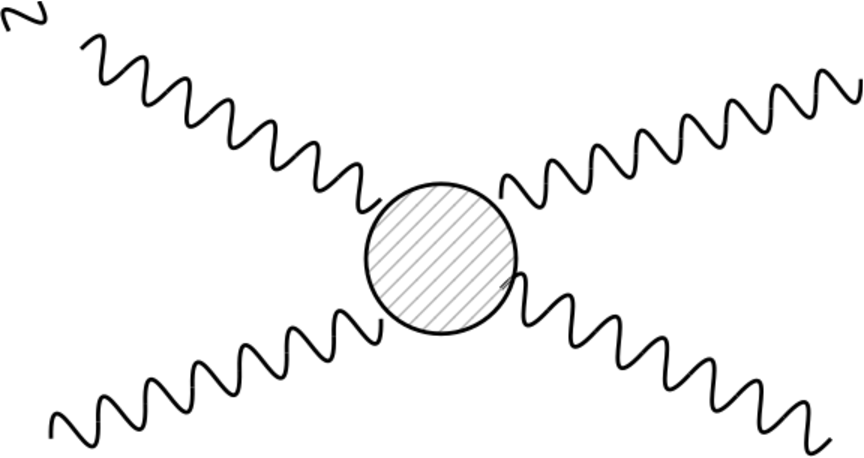
\includegraphics[scale=0.2]{figs/pc3.pdf}    & Actually finite (gauge invariance)                                                                    \\ 
0     & 2     & 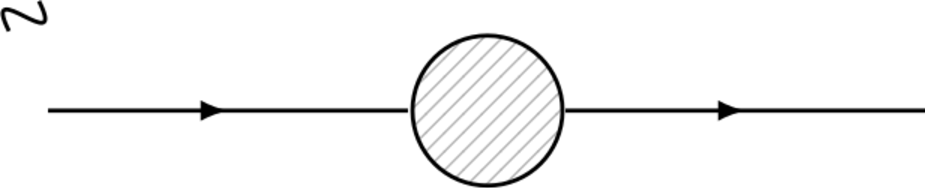
\includegraphics[scale=0.2]{figs/pc4.pdf}  & $\bar{\psi}\slashed{\partial}\psi + \bar{\psi}m\psi$, i.e. $Z_2$ and $Z_m$                            \\
2     & 1     & 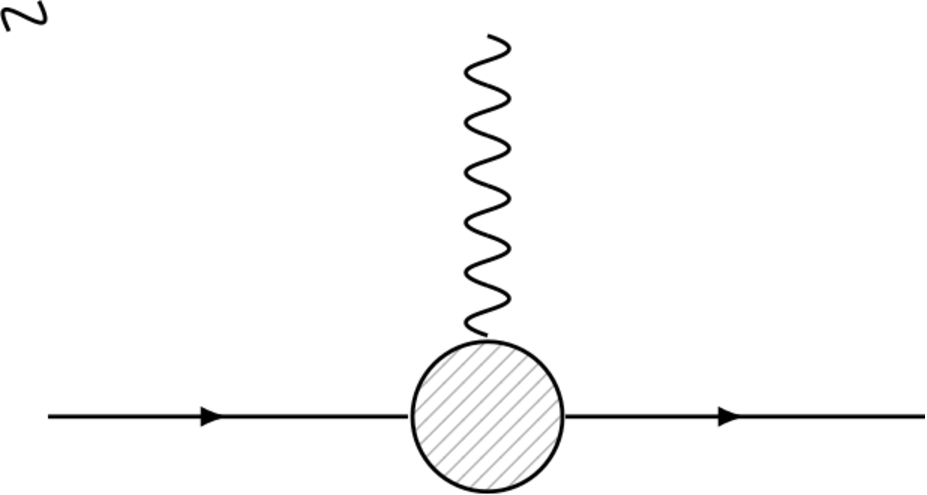
\includegraphics[scale=0.2]{figs/pc5.pdf} & 
$\bar{\psi}\slashed{A}\psi$, i.e. $Z_1$
\end{tabular}
\end{table}
In summary, QED is power-counting renormalisable. Note that if $E_F=4$ and $E_B=0$ then $D=-2$, i.e. the the four-fermion vertex is convergent.

Now let's move on from QED and consider $\mathcal{L}_{4F}$ instead. We can write the expression
\begin{equation}
2I_F + E_F = 4V
\end{equation}
so, if we only have fermions
\begin{equation}
\begin{split}
D &= \frac{3}{2}(4V-E_F) - 4V + 4 \\
&= 4 + 2V - \frac{3}{2} E_F.
\end{split}
\end{equation}
In other words,
\begin{enumerate}
\item every time we add a vertex, the graph becomes \textit{more} divergent
\item graphs with \textit{any} number of external fermions will diverge at a high enough order.
\end{enumerate}
For example, if $E_F = 6$, there are divergences for $V=3$. So $\mathcal{L}_{4F}$ is non-renormalisable. Adding bosons doesn't help the situation; we can trace the problem again to $[G_F]=-2$. 
\newline
\newline
\textbf{Theorem: } A theory is only power counting renormalisable if all the couplings have mass dimension $\geq 0$.
\newline
\textbf{Proof: } Consider a vertex $V_{bf}$ with $b$ boson lines, $f$ fermion lines and $p$ derivatives. The corresponding term in the Lagrangian is $g\phi^b\psi^f\partial^p$. The dimension of the coupling is
\begin{equation}
d_{bf}^p = 4 - b - \frac{3}{2}f - p
\end{equation}
because $[\mathcal{L}]=4$, $[\phi]=[A]=1$, $[\psi]=3/2$ and $[\partial]=1$. However,
\begin{equation}
\begin{split}
2I_B + E_B &= \sum bV_{bf}^p \\
2I_F + E_F &= \sum fV_{bf}^p \\
\text{so } D &= \sum bV_{bf}^p - E_B + \frac{3}{2}\big(\sum fV_{bf}^p - E_F\big) - 4 \sum V_{bf}^p + 4 + \sum p V_{bf}^p \\
&= \sum\big(b + \frac{3}{2}f + p - 4\big)V_{bf}^p - E_B - \frac{3}{2}E_F + 4 \\
&= -\sum d_{bf}^pV_{bf}^p - E_B - \frac{3}{2}E_F + 4.
\end{split}
\end{equation}
This means that for renormalisability we need $d_{bf}^p \geq 0$ so that $D$ increases as $V$ increases.
\newline
\textbf{Corollary: } For a theory with scalar, fermion and vector fields, the only vertices allowed in a renormalisable Lorentz invariant Lagrangian are:
\begin{table}[h!]
\begin{tabular}{ll}
 Pure scalar & $\phi^3$, $\phi^4$  \\
 Yang-Mills &  $\partial_\mu A_\nu A^\mu A^\nu$, $A_\mu A_\nu A^\mu A^\nu$ \\
 Gauge-scalar interactions & $\phi A_\mu A^\mu$, $\phi^2 A_\mu A^\mu$, $\phi \partial_\mu \phi A^\mu$ \\
 Yukawa &  $\phi \bar{\psi} \psi$ \\
 Gauge interactions & $\bar{\psi} \slashed{A} \psi$
\end{tabular}
\end{table}
\newline
\textbf{Proof: } $d^p_{bf} \geq 0$ only for the above. Note
\begin{itemize}
\item you need at least three fields
\item $A_\mu A^\mu A^\nu$, $\phi^2 \partial_\mu \phi$ and $\phi^2 A_\mu$ are not Lorentz invariant.
\end{itemize}
%
\subsection{Intermediate vector bosons}
%
Power counting renormalisability, chirality and Lorentz invariance suggest a vertex of the form $g\bar{\psi}_L\slashed{A}\psi_L$. Such a coupling is dimensionless so, following arguments from the previous section, unitarity is possible. This is the only possible coupling for left-handed fermions: the Yukawa coupling $\phi \bar{\psi}\psi = \phi(\bar{\psi}_L\psi_R + \bar{\psi}_R\psi_L)$ so is not a left-handed-only coupling. The charged currents are
\begin{equation}
\begin{split}
\frac{1}{2}J_\mu &= \bar{\nu}_e\gamma_\mu e_L + ... + \bar{u}_L \gamma_\mu d^\prime_L + ... \qquad \Delta Q = +1 \\
\frac{1}{2}J_\mu^\dagger &= \bar{e}_L \gamma_\mu \nu_e + ... + \bar{d}^\prime_L \gamma_\mu u_L + ... \qquad \Delta Q = -1
\end{split}
\end{equation}
so we need \textit{two} charged vector fields 
\begin{equation}
W_\pm^\mu = \frac{1}{\sqrt{2}} (W_1^\mu \pm i W_2^\mu)
\end{equation}
where $W_1^\mu$ and $W_2^\mu$ are real. Equivalently, we could define one complex field $W^\mu$, such that $W_+^\mu = W^\mu$ and $W_-^\mu = W^{\mu \dagger}$. The charged current Lagrangian can be written
\begin{equation}
\begin{split}
\mathcal{L}_{CC} &= \frac{g}{2\sqrt{2}}(J_\mu^\dagger W^\mu + W_\mu^\dagger J^\mu) \\
&= \frac{g}{\sqrt{2}}\bar{\nu}_e \slashed{W} e_L + \frac{g}{\sqrt{2}}\bar{e}_L \slashed{W}^\dagger \nu_e + ...
\end{split}
\end{equation}
where the factor of $2\sqrt{2}$ is conventional. $g$ is the (real) dimensionless coupling, and is the same for every term in $J_\mu$ (universality). 

$W_\mu$ is different from the $A_\mu$ in electromagnetism: 
\begin{itemize}
\item $W_\mu$ is charged, and thus complex
\item $W_\mu$ must be massive, because CC weak interactions are short range
\end{itemize}
In 1936 the Romanian physicist Alexandru Proca wrote down a Lagrangian to describe $W^\mu$, consisting of a kinetic term and a mass term:
\begin{equation}
\begin{split}
\mathcal{L}_W &= - \frac{1}{2}(\partial_\mu W_\nu - \partial_\nu W_\mu)^\dagger(\partial^\mu W^\nu - \partial^\nu W^\mu) + m_W^2 W_\mu^\dagger W^\mu \\
&\equiv -\frac{1}{2}W_{\mu \nu}^\dagger W^{\mu \nu} + m_W^2 W_\mu^\dagger W^\mu .
\end{split}
\end{equation}
So this gives an equation of motion
\begin{equation}
\begin{split}
&(\partial^2 + m_W^2) W^\mu - \partial^\mu \partial^\nu W_{\mu \nu} = 0 \\
&\implies \partial_\mu W^\mu =0 \text{ if } m_W \neq 0.
\end{split}
\end{equation}
We can look for plane wave solutions of the form $W^\mu = \epsilon^\mu e^{-i k \cdot x}$:
\begin{equation}
\begin{split}
(-k^2 + m_W^2)\epsilon^\mu + k^\mu k_\mu \epsilon^\nu &= 0 \\
\implies m_W^2 k_\mu \epsilon^\mu &= 0 
\end{split}
\end{equation}
where we have taken the physical solution in the last line. Since $W$ is massive it has three spin states: in the rest frame $k^\mu = (m_W, 0)$
\begin{equation}
\begin{split}
\epsilon_r^\parallel &= (0, \underline{\epsilon}_r) \qquad r=1,2,3 \\
\text{where } \qquad \underline{\epsilon}_1 &= (1,0,0) \\
\underline{\epsilon}_2 &= (0,1,0) \\
\underline{\epsilon}_3 &= (0,0,1). 
\end{split}
\end{equation}
$\underline{\epsilon}_1$ and $\underline{\epsilon}_2$ are the transverse components and can be combined to form $\underline{\epsilon}_\pm = \frac{1}{\sqrt{2}}(1, \pm i, 0)$, and $\underline{\epsilon}_3$ is the longitudinal component. 

So if $k^\mu = (E, 0, 0, k)$, $\epsilon_3 = \frac{1}{m_W}(k,0,0,E)$. N.B. for $E \gg m_W$, $\epsilon_3 \approx k^\mu/m_W + \mathcal{O}(m_W/E)$. Now let's evaluate the different polarisation sums: defining $\epsilon_0^\mu = k^\mu/m_W$ (so in the rest frame $\epsilon_0^\mu = (1, \underline{0})$ which is timelike, and therefore unphysical)
\begin{equation}
\begin{split}
&\sum_{r=0,1,2,3}\eta^{rr}\epsilon_r^\mu \epsilon_r^{\nu *} = - \eta^{\mu \nu} \qquad \text{completeness: cf RQFT} \\
\text{so } &\sum_{r=1,2,3}\epsilon^\mu_r \epsilon_r^{\nu *} = -\eta^{\mu \nu} + \epsilon_0^\mu \epsilon_0^\nu = -\eta^{\mu\nu} + \frac{k^\mu k^\nu}{m_W^2}
\end{split}
\end{equation}
The propagator is 
\begin{equation}
\Delta^{\mu\nu}_W = \frac{i(-\eta^{\mu \nu} + k^\mu k^\nu/m_W^2)}{k^2-m_W^2 + i\epsilon}
\end{equation}
because
\begin{equation}
\big((-k^2 + m_W^2)\eta_{\mu\nu} + k_\mu k_\nu)\Delta^{\nu \rho}_W = -i\delta_\mu^\rho
\end{equation}
(check this as an exercise).

The Feynman rule for the interaction is
\newline
\begin{wrapfigure}{l}{0.4\linewidth}
  \centering
  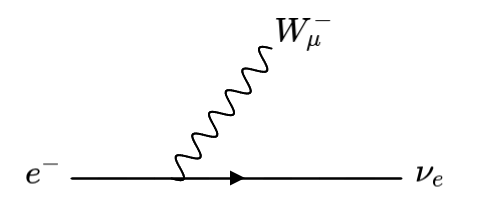
\includegraphics[width=\linewidth]{figs/17a.png}
\end{wrapfigure}
\begin{equation}
i\frac{g}{\sqrt{2}}\gamma_\mu\frac{1}{2}(1-\gamma^5)
\end{equation}
How does this theory work in practice? The following are some examples.
\newline
\newline
\subsubsection{$\mu^- \to e^-\bar{\nu}_e\nu_\mu$}
%\begin{wrapfigure}{r}{0.4\linewidth}
%  \centering
  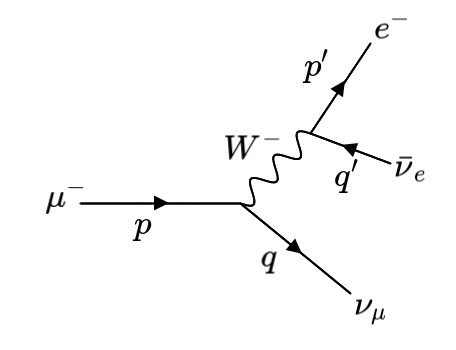
\includegraphics[width=0.4\linewidth]{figs/17b.png}
%\end{wrapfigure}
The momentum of $W^-$, $k=p-q=p^\prime + q^\prime$.
\begin{equation}
\begin{split}
\mathcal{M}& = \frac{(ig)^2}{8}\bar{u}(p^\prime)\gamma_mu(1-\gamma^5)v(q^\prime)\frac{(-\eta^{\mu \nu} + k^\mu k^\nu/m_W^2)}{k^2-m_W^2}\bar{u}(q)\gamma_\nu(1-\gamma^5)u(p) \\
\text{But } \qquad &\bar{u}(q)\slashed{k}(1-\gamma^5)u(p) = \bar{u}(q)(\slashed{p}-\slashed{q})(1-\gamma^5)u(p) = m_\mu \bar{u}(q)(1+\gamma^5)u(p) \\
&\bar{u}(p^\prime)\slashed{k}(1-\gamma^5)v(q^\prime) = \bar{u}(p^\prime)(\slashed{p}^\prime+\slashed{q}^\prime)(1-\gamma^5)v(q^\prime) = -m_e \bar{u}(p^\prime)(1+\gamma^5)v(q^\prime) 
\end{split}
\end{equation}
so the $k^\mu k^\nu/m_W^2$ term in the propagator tends to $m_e m_\mu/m_W^2 \sim 10^{-8}$ ($m_W=75$ GeV). Also $k^2 = m_\mu^2 - 2p \cdot q < m_\mu^2 \ll m_W^2$. If we ignore these terms, 
\begin{equation}
\frac{1}{2}\sum_{spins}|\mathcal{M}|^2 = \frac{2g^4}{m_W^4}(p \cdot q^\prime)(p^\prime \cdot q)
\end{equation}
i.e. this is the same as in 4-Fermi theory, provided that $G_F/\sqrt{2} = g^2/8m_W^2$. So the weak force is weak because $m_W$ is large ($\gg 1$ GeV). It is easy to see that the same arguments apply to \textit{all} weak decays in Chapter 1. 
%
\subsubsection{$\nu_\mu e^- \to \mu^- \nu_e$}
%
%\begin{wrapfigure}{r}{0.4\linewidth}
%  \centering
  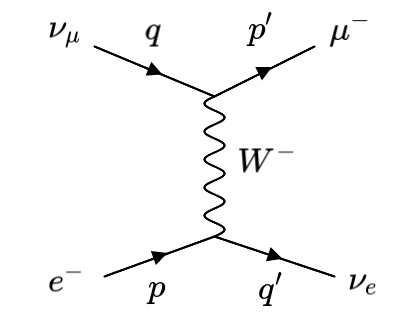
\includegraphics[width=0.3\linewidth]{figs/17c.png}
%\end{wrapfigure}
Here $k = p=q^\prime = p^\prime - q$ and
\begin{equation}
\mathcal{M} = \frac{(ig)^2}{8}\bar{u}(q^\prime)\gamma_\mu(1-\gamma^5)u(p)\frac{i(-\eta^{\mu\nu} + k^\mu k^\nu/m_W^2)}{k^2-m_W^2}\bar{u}(p^\prime)\gamma_\nu (1-\gamma^5)u(q).
\end{equation}
As before, $k^\mu k^\nu /m_W^2 \to m_e m_\mu /m_W^2$ so we can ignore these terms. But $k^2 = (p-q^\prime)^2 = t$ so
\begin{equation}
\frac{d\sigma}{d\Omega} = \frac{g^4}{128\pi^2}\frac{s}{(t-m_W^2)^2}
\end{equation}
where $s=4E^2$ and $t=-4E^2\sin^2\theta/2$. Integrating over $\phi$,
\begin{equation}
\begin{split}
\frac{d\sigma}{d\cos\theta} &= \frac{g^4E^2}{64\pi(E^2\sin^2\theta/2 + m_W^2/4)^2}
\\
&= \frac{g^4}{64\pi E^2}\csc^2 \frac{\theta}{2}\bigg( 1 + \mathcal{O}\big(\frac{m_W^2}{E^2}\big)\bigg).
\end{split}
\end{equation}
At very high energy, $E^2 \gg m_W^2$ so unitarity is restored. 
%
\subsubsection{$\nu \bar{\nu} \to W^+ W^-$}
%
Consider now the production of external $W^\pm$. In this case $q + q^\prime = k + k^\prime$. 
\newline
%
%\begin{wrapfigure}{r}{0.4\linewidth}
%  \centering
  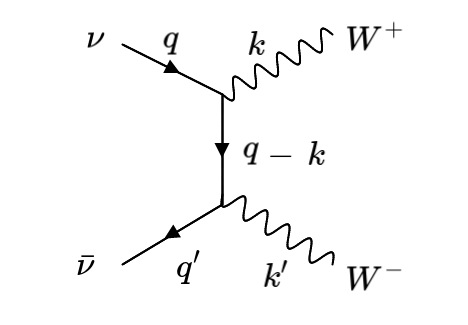
\includegraphics[width=0.4\linewidth]{figs/18a.png}
%\end{wrapfigure}
%
\begin{equation}
\mathcal{M} = \frac{(ig)^2}{8} \bar{v}(q^\prime) \gamma_\mu(1-\gamma^5)\frac{i(\slashed{q}-\slashed{k}+m_e)}{(q-k)^2 -m_e^2}\gamma_\nu(1-\gamma^5)u(q)\epsilon_r^\mu(k^\prime)^* \epsilon_r^\nu(k).
\end{equation}
We want the behaviour of the cross-section at very high energy, so we can ignore $m_e$. Also consider the $W$s to be longitudinally polarised, i.e. $\epsilon_3^\mu(k) \approx k^\mu/m_W + \mathcal{O}(m_W/E)$. So
\begin{equation}
\mathcal{M} = \frac{-ig^2}{4}\frac{1}{m_W^2(q-k)^2}\bar{v}(q^\prime)\slashed{k}^\prime(\slashed{q}-\slashed{k})\slashed{k}(1-\gamma^5)u(q)
\end{equation}
But $\slashed{q}u(q)=0$ so 
\begin{equation}
\begin{split}
\slashed{k}u(q) &= - (\slashed{q}-\slashed{k})u(q) \\
\text{similarly } \qquad \bar{v}(q^\prime)\slashed{k}^\prime &= \bar{v}(q^\prime)(\slashed{q}-\slashed{k})
\end{split}
\end{equation}
since$\slashed{q}u(q)=0$, writing $p = q -k$ ,
\begin{equation}
\begin{split}
\mathcal{M} &= \frac{-ig^2}{4}\frac{1}{m_W^2p^2}\bar{v}(q^\prime)\slashed{p}\slashed{p}\slashed{p}(1-\gamma^5)u(q) \\
&= +\frac{ig^2}{4}\bar{v}(q^\prime)\slashed{k}(1-\gamma^5)u(q)
\end{split}
\end{equation}
and
\begin{equation}
\begin{split}
    \sum_{pol}|\mathcal{M}|^2 &= \frac{g^4}{16 m_W^4}\ tr\bigg(\slashed{q}^\prime \slashed{k}(1-\gamma^5)\slashed{q}\slashed{k}(1-\gamma^5)\bigg) \\
    & = \frac{g^4}{2m_W^4}(2q^\prime \cdot k q \cdot k - k^2 q \cdot q^\prime) \\
    & = \frac{g^4}{m_W^4} (q \cdot k q^\prime \cdot k - \frac{m_W^2}{2}q \cdot q^\prime).
\end{split}
\end{equation} 
Transforming to the Mandelstam variables, we can write
\begin{equation}
\begin{split}
s &= 2 q \cdot q^\prime, \\
t &= - 2 q \cdot k + m_W^2, \\
u &= - 2 q^\prime \cdot k + m_W^2,
\end{split}
\end{equation}
so
\begin{equation}
\begin{split}
    \sum_{pol}|\mathcal{M}|^2 &= \frac{g^4}{4m_W^4} \big(m_W^4 - (u + t + s)m_W^2 + ut\big)\\
    &= \frac{g^4}{4m_W^4} \big(m_W^4 - 2m_W^2 \times m_W^2 + ut\big)\\
 \text{so} \qquad   \frac{d\sigma}{d\Omega} &= \frac{g^4}{64\pi^2m_W^4}\frac{ut-m_W^4}{4s}.
\end{split}
\end{equation}
Considering the high energy limit, $E^2 \gg m_W^2$, so we can neglect the $m_W^4$ term, $s=4E^2$ and $ut = 4E^2\sin(\theta/2)\times 4E^2\cos(\theta/2) = 4E^4\sin^2\theta$. Integrating over $\phi$ in this limit,
\begin{equation}
\begin{split}
\frac{d\sigma}{d\cos\theta} &= \frac{g^4}{128\pi}\frac{E^2}{m_W^4}\sin^2\theta \\
\text{and} \qquad \qquad \sigma &= \frac{g^4}{128\pi}\frac{E^2}{m_W^4} \int_{-1}^1 d\cos\theta (1-\cos^2\theta) \\
&= \frac{g^4}{96\pi}\frac{E^2}{m_W^4}. 
\end{split}
\end{equation}
We can see that this violates unitarity! The cross section is unbounded as $E \to \infty$. It is clear that the $k_\mu k_\nu/m_W^2$ term in the $W$ propagator will spoil the power-counting renormalisability for graphs with internal $W$ lines coupled to internal fermions. 
%
\begin{wrapfigure}{l}{0.4\linewidth}
  \centering
  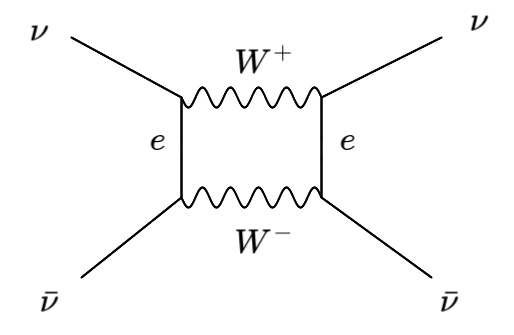
\includegraphics[width=\linewidth]{figs/18b.png}
\end{wrapfigure}
%
For example, this diagram has contributions
\begin{equation}
\sim \int d^4k \bigg(\frac{k^2/m_W^2}{k^2-m_W^2}\bigg)^2 \bigg(\frac{\slashed{k}}{k}\bigg)^2 \sim \int \frac{d^4k}{m_W^4k^2}.
\end{equation}
Unitarity and renormalisability of theories with vectors requires \textit{gauge invariance} under $W_\mu \to W_\mu + \partial_\mu \alpha \implies \epsilon_\mu \to \epsilon_\mu + \alpha k_\mu$. 
Remember that this problem doesn't arise in QED because for the comparative process $\gamma e^- \to \gamma e^-$ (or, by crossing, $e^+e^- \to \gamma \gamma$) we have two contributing diagrams:

%
%\begin{wrapfigure}{r}{0.7\linewidth}
%  \centering
  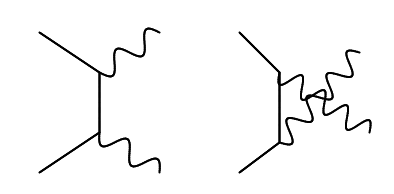
\includegraphics[width=0.8\linewidth]{figs/18c.png}
%\end{wrapfigure}
%
\newline
whereas for EW, $W^+ \neq W^-$ so there is only one.

%
%\begin{wrapfigure}{r}{0.7\linewidth}
%  \centering
  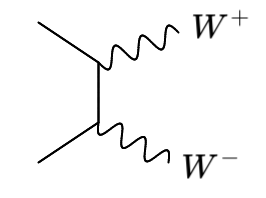
\includegraphics[width=0.3\linewidth]{figs/18d.png}
%\end{wrapfigure}
%
